\documentclass{article}
\usepackage{amsmath}
\usepackage{graphicx}
\usepackage{float}
\usepackage{hyperref}
\usepackage{fancyvrb}
\usepackage{matlab-prettifier}
\usepackage{enumitem}
% \usepackage{minted}
\usepackage{palatino}
\fontfamily{SansSerif}

\setlength{\parindent}{0pt}

\title{EE324: Control Systems Lab \\ Experiment 1: DC Motor Position Control\\ \textbf{Group 1 - Thursday}}
\author{\large Harsh S Roniyar\\ \large 22B3942 \and \large Pranav Prakash\\ \large 22B3945 \and \large Aman Verma\\ \large 22B3929}

\begin{document}

\maketitle

\section{Objective}
To design and implement a PID position controller using Arduino Mega for a DC motor.

The specific objectives were:
\begin{itemize}
\item To rotate the dc motor by an angle of $180^{\circ}$ from any given point. 
\item To ensure that the task is constrained by the design specifications of rise time $t_r = 0.5s$, settling time $t_s = 1s$ and 10\% overshoot.
\end{itemize}

\section{Control Algorithm}

The control algorithm used in this experiment is a PID controller. The PID controller is given by the following equation:
\begin{equation}
u(t) = K_p e(t) + K_i \int_{0}^{t} e(\tau) d\tau + K_d \frac{de(t)}{dt}
\end{equation}

where $u(t)$ is the control input, $e(t)$ is the error signal, $K_p$, $K_i$ and $K_d$ are the proportional, integral and derivative gains respectively.

\clearpage

Some important code snippets below shows the implementation of the PID position controller in Arduino.
\begin{lstlisting}[style=Matlab-Pyglike,breaklines=true,postbreak=\mbox{\textcolor{red}{$\hookrightarrow$}\space}, language=C++, escapeinside={(*@}{@*)}]
/*
  Experiment 1 : DC Motor Control

  Group 1:
  22B3929 - Aman Verma
  22B3942 - Harsh S Roniyar
  22B3945 - Pranav Prakash
*/

#define RANGE_DIFF 3
#define ERROR_RANGE_HIGH 6
#define ERROR_RANGE_LOW -6

int ctrl_a = 5;
int ctrl_b = 6;
int potpin = A0;

(*@{\raisebox{-1pt}[0pt][0pt]{$\vdots$}}@*)

float p = 5.55;
float i = 0.0224;
float d = 5.89;

(*@{\raisebox{-1pt}[0pt][0pt]{$\vdots$}}@*)

void control_motor(char d, int speed) {
  if (d == 's') {
    analogWrite(ctrl_a, 0);
    analogWrite(ctrl_b, 0);
  } else if (d == 'f') {
    analogWrite(ctrl_a, 0);
    analogWrite(ctrl_b, speed);
  } else {
    analogWrite(ctrl_a, speed);
    analogWrite(ctrl_b, 0);
  }
}

void setup() {
  Serial.begin(9600);
  pinMode(potpin, INPUT);
  pinMode(ctrl_a, OUTPUT);
  pinMode(ctrl_b, OUTPUT);

  read_pot_val();
  init_val = new_val;
  find_non_linear();

  fin_val = int(180 + init_val);

  if(fin_val > 350){
    fin_val = int(init_val - 180);
  }

  update_dir(fin_val - init_val);
}

void loop() {
  read_pot_val();
  
  error = float(fin_val-new_val); 
  integrate = integrate + error;
  tot_err = p*error + i*integrate + d*(error-preverror);
  preverror=error;

  if(start == 0){
    start = millis(); 
  }
  
  if(tot_err<0){
    control_motor('b',(min(abs(tot_err),255)));
  } else {
    control_motor('f',(min(abs(tot_err),255)));   
  } 

  Serial.print(millis() - start);
  Serial.print(",");
  Serial.println(new_val);
}
\end{lstlisting}

% \clearpage
\section{Challenges Faced and Solutions}
\begin{itemize}%[nolistsep]
    \item \textbf{Tuning of the PID Gains:} Finding the appropriate values for the PID gains ($K_p$, $K_i$, $K_d$) to meet the design specifications was challenging.\\
    \underline{\textit{Solution:}} Started with a proportional-only controller, then introduced integral and derivative gains gradually, fine-tuning based on the observed response.

    \item \textbf{Non-linearities in the Potentiometer:} The potentiometer used to measure the motor's position had a non-linear response in a certain region, affecting position control accuracy.\\
    \underline{\textit{Solution:}} Identified non-linear regions by analyzing the potentiometer output across its range. 

    \item \textbf{Overshoot and Stability Issues:} Achieving a balance between a fast response (low rise time) and minimal overshoot was difficult. Over-tuning for speed lead to excessive overshoot or instability.
    \underline{\textit{Solution:}} Gradually tuned the derivative gain ($K_d$) to dampen oscillations and reduce overshoot while maintaining a quick response. Monitored the system's step response closely during tuning to prevent instability.
\end{itemize}

\section{Results}

\begin{itemize}[nolistsep]
    \item The non-linear region was found to be between $25^{\circ}$ and $35^{\circ}$.
    \item The final values of the PID gains were $K_p = 5.55$, $K_i = 0.0224$ and $K_d = 5.89$.
    \item The rise time was found to be 0.41s, settling time was found to be 0.993s and the overshoot was found to be 3\%.
    \item The analog reading of potentiometer corresponding to a swing of $180^{\circ}$ was found to be 506.
    \item The output of the motor position vs time is shown in the below graph.
    \begin{figure}[!htb]
        \centering
        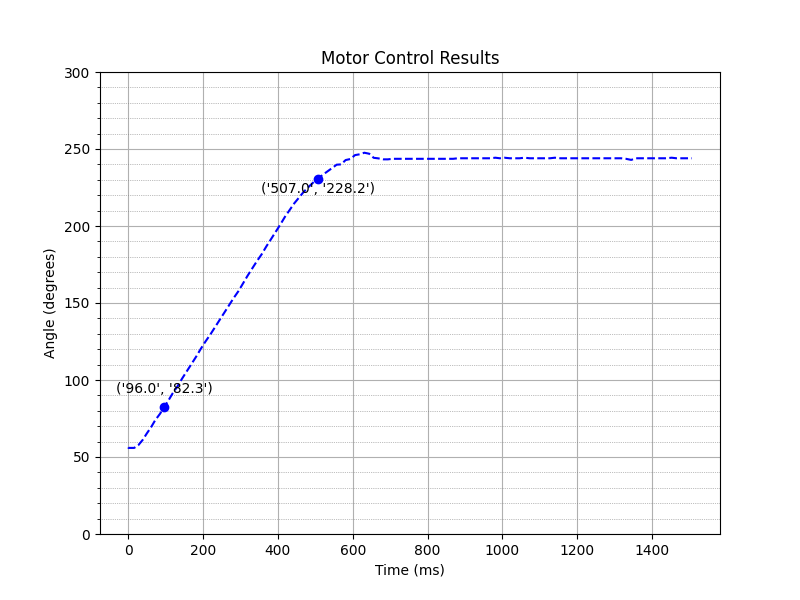
\includegraphics[width=0.8\textwidth]{../././motor_control.png}
        \caption{Motor Position vs Time}
        \label{fig:plot}
    \end{figure}
\end{itemize}

\section{Observations and Inference}
\begin{itemize}[nolistsep]
    \item The PID controller was able to rotate the motor by $180^{\circ}$ from any given point.
    \item The rise time, settling time and overshoot were found to be within the design specifications.
    \item The potentiometer reading corresponding to a swing of $180^{\circ}$ was not exactly 512 as expected. This was due to the non-linear region of the potentiometer.
\end{itemize}

\section{TA Result Sheet}

\begin{center}
    \includegraphics[width=0.8\textwidth]{../././TASheet.jpg}
\end{center}

\end{document}